\chapter{工具设计与实现}
本章中将主要介绍如何将补丁版本迁移、语义影响范围分析、冲突分析等过程具体实现之,并组合成整体流程。

\section{整体架构}

\section{补丁版本迁移}

如前所述,补丁版本迁移主要用于解决问题\ref {patch_reversion}。我们在实现该过程时,主要采用了git工具和Beyond Compare工具来实现版本合并和冲突解决的过程。

我们下面将利用git的分支功能进行版本合并。首先介绍一些前提假设:

\begin{enumerate}
	\item 假设git的工作目录如图\ref {git_work_dir}所示。其中git\_working\_dir为git目录,下属目录包括源代码仓库src和git目录的隐藏文件夹.git。另外与git目录平级的目录patch下面则存储了具体的补丁文件。

	\item 假设补丁$p_1 = old.patch$,并且采用git diff或其他Unix diff命令生成。
\end{enumerate}

\begin{figure}[H]
	\centering
	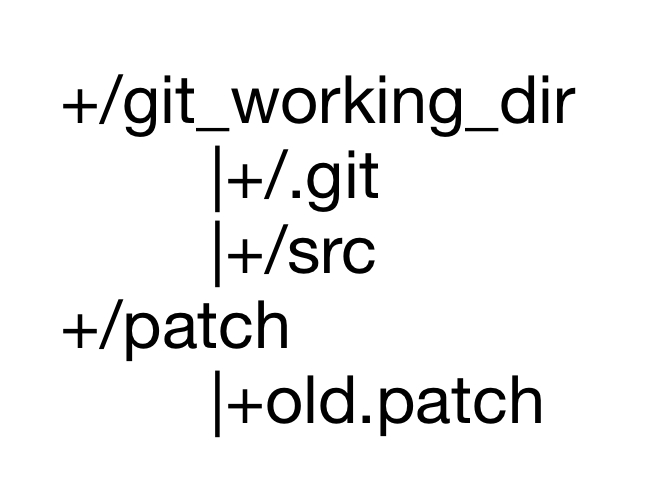
\includegraphics{chap04_work_dir}
	\caption {git工作目录}
	\label {git_work_dir}	
\end{figure}

下面将具体介绍整个版本合并的过程。


首先在工作目录下将git切换到主分支master。然后在主分支master中提交代码版本$v_1$。

\begin{lstlisting} [style=BashInputStyle]
git checkout master
git add .
git commit -a -m "old version committed"
\end{lstlisting}

然后新建并切换到分支new中,并提交代码版本$v_2$。
\begin{lstlisting} [style=BashInputStyle]
git checkout -b new
git add .
git commit -a -m "new version committed"
\end{lstlisting}

再次从主分支新建并切换到分支patch,然后将补丁$p_1$应用到版本$v_1$,获得旧版本应用补丁后的代码,其版本为$v_3$,并提交代码版本$v_3$。此时我们所应用的补丁$p_1$是专为版本$v_1$设计,所以应用时不会出现问题。

\begin{lstlisting} [style=BashInputStyle]
git checkout master
git checkout -b patch
git apply ../patch/old.patch
git add .
git commit -a -m "patched version from old version committed"
\end{lstlisting}

然后再切换回分支new,将分支patch合并入分支new,获得新版本应用补丁后的代码,其版本为$v_4$,并使用Beyond Compare工具解决可能出现的冲突问题。将冲突解决完毕后,再提交版本$v_4$。

\begin{lstlisting} [style=BashInputStyle]
git checkout new
git merge patch
git mergetool
git commit -a -m "patched version from new version committed"
\end{lstlisting}

如果确实有冲突,那么git mergetool命令会调用第三方的可视化合并工具并引导你去解决冲突。这里我们采用的合并工具即为Beyond Compare,它会展开一个可视化的界面,并给出冲突位置的提示,方便进行人工选择、合并。

整个过程可以参考图\ref {git_merge}。

\begin{figure}[H]
	\centering
	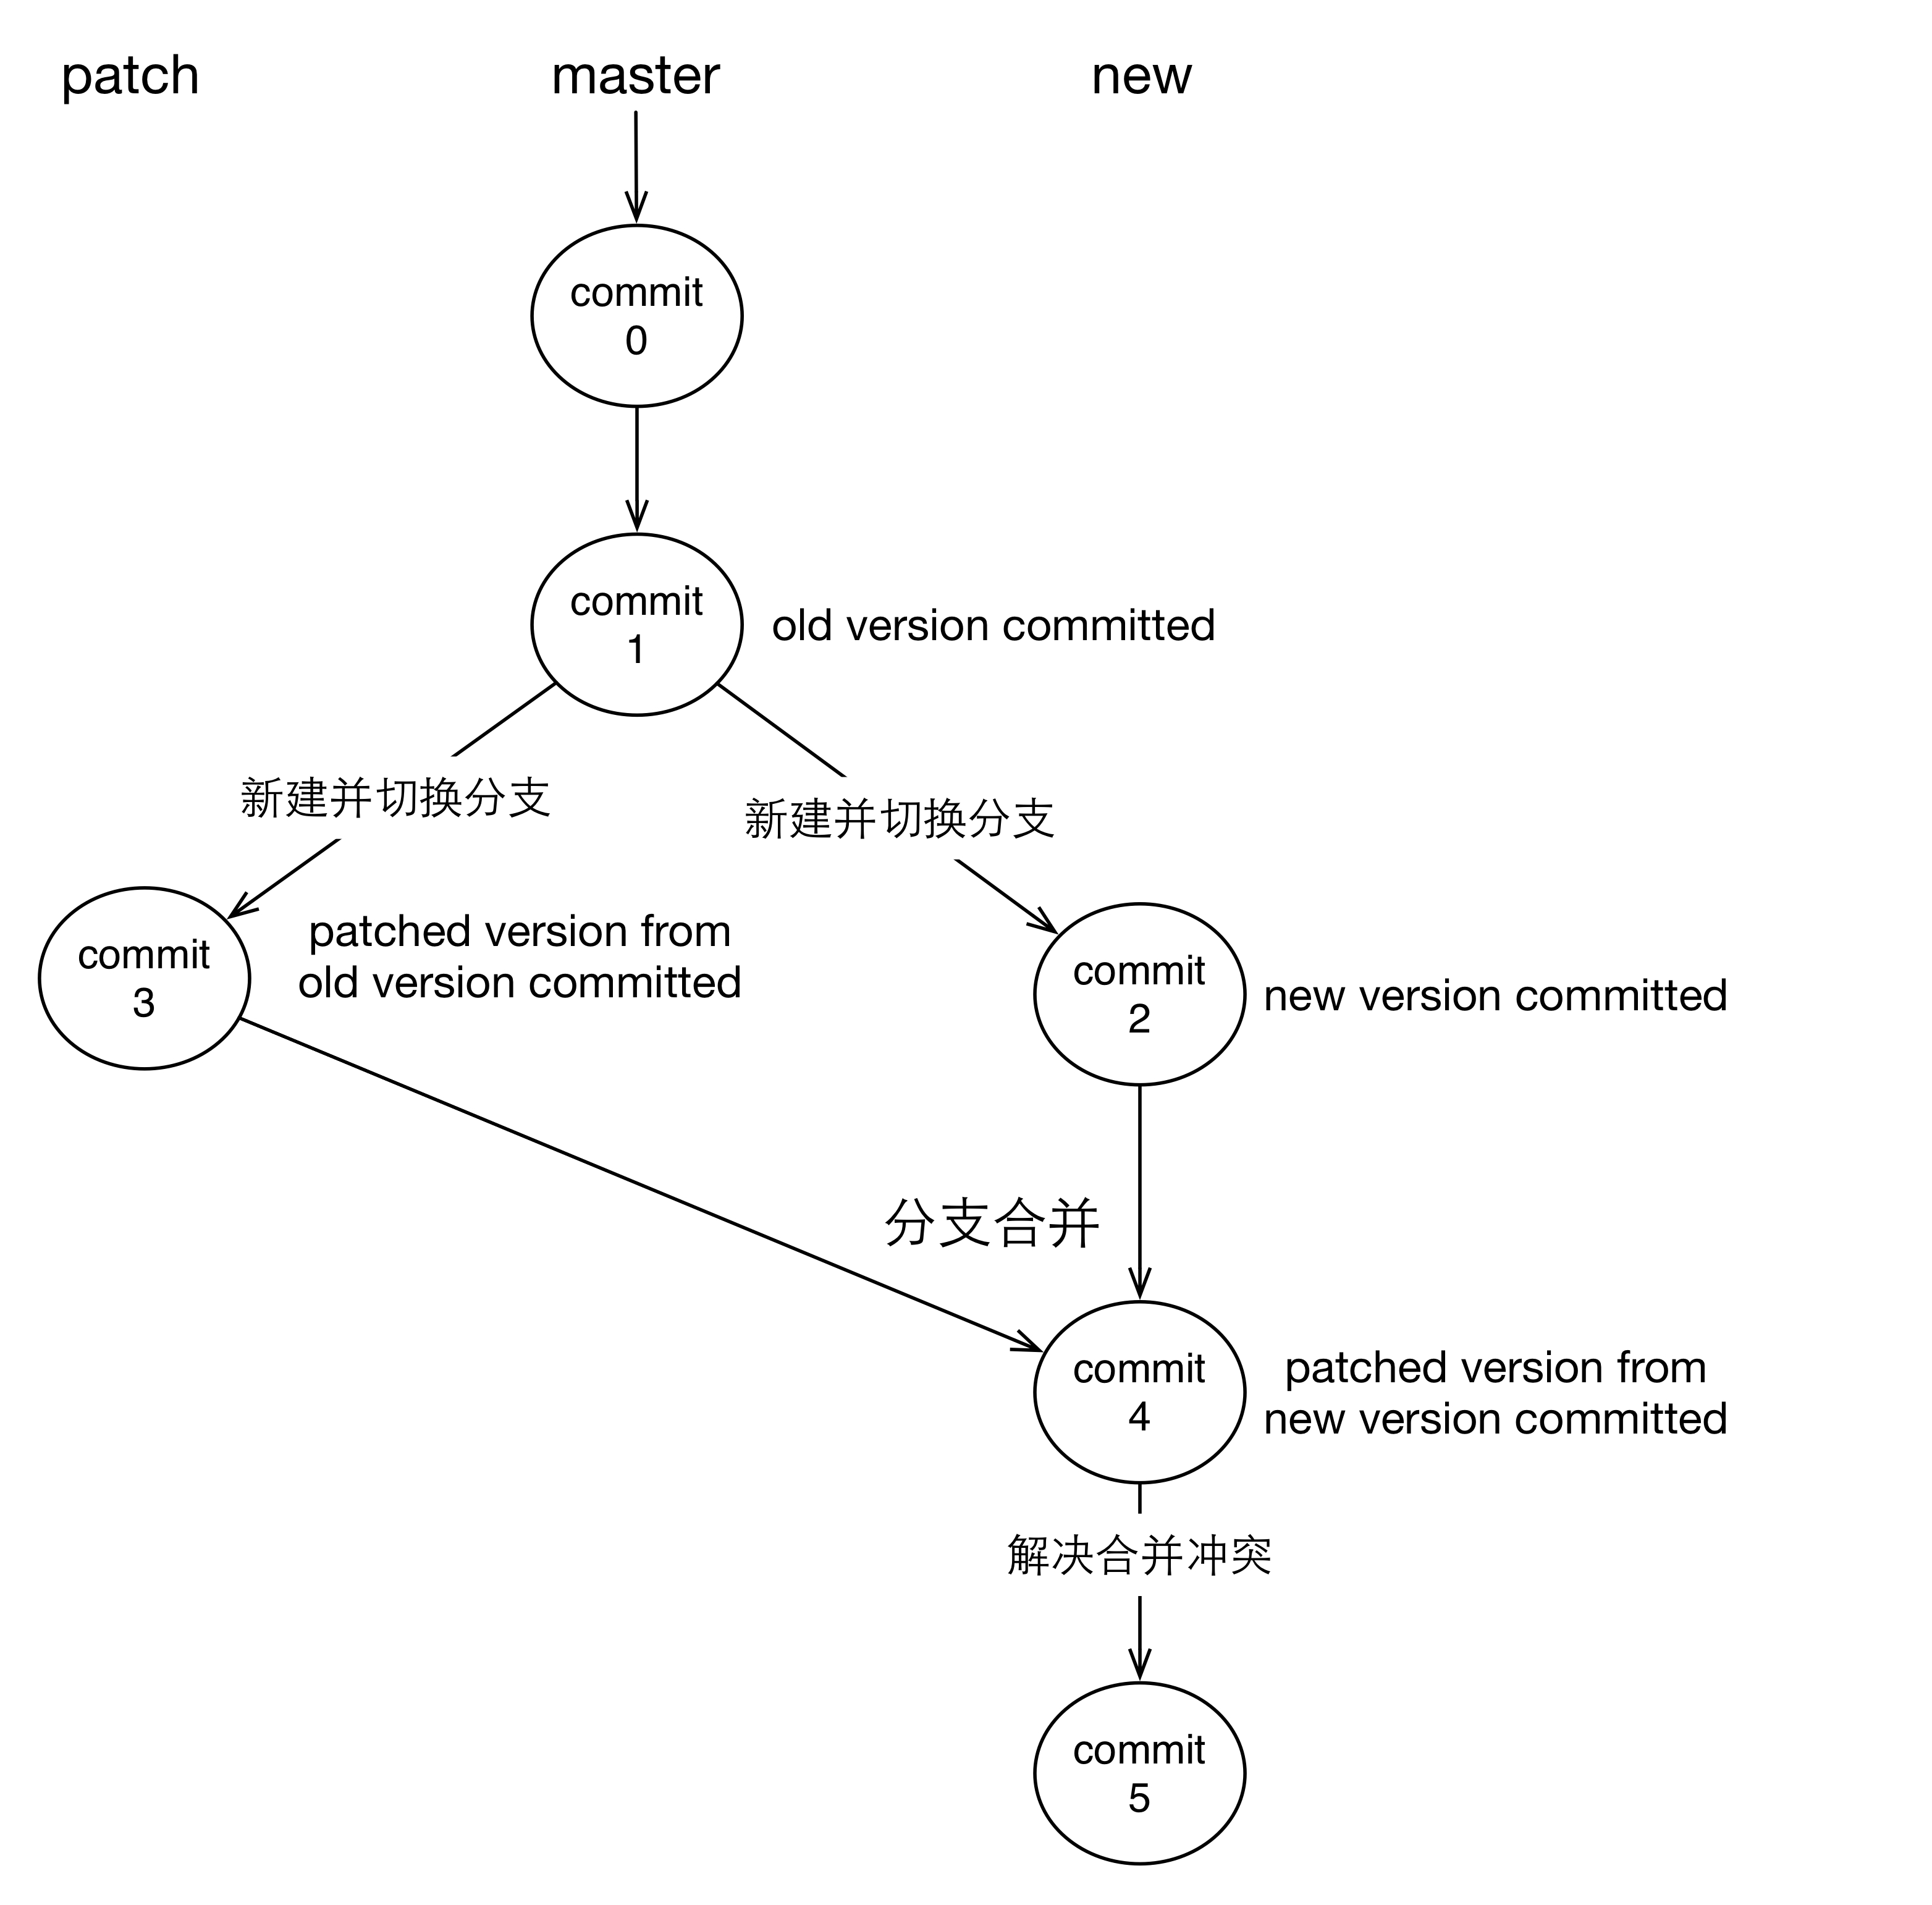
\includegraphics[width=.9\columnwidth]{chap04_git_merge}
	\caption {git版本合并}
	\label {git_merge}	
\end{figure}

\section{语义影响范围分析}

如前所述,语义影响范围分析主要用于解决问题\ref {impacted_area}。语义影响范围分析需要首先定义好影响范围和影响元素的级别。在实际情况中,我们主要采用了较为简单的分析过程,即将影响范围限制在方法内部,但是将受影响元素设置为程序语句级别,以保证精度。

由于我们采用了现有工具来完成具体的程序间差异分析和变更影响分析过程,因而这两个子过程的分析算法已经无需我们自己实现。我们可以将主要精力放在如何整合两个子过程的工作上,并将其工具转化为适用于本问题的具体情况。

在具体的实现过程中,我们发现一些主要需要解决的问题包括:
\begin{enumerate}
	\item 修正ASTro的分析结果,以提高精确度。
	\item 改进jpf-regression工具,包括:
		\begin{enumerate}
			\item 修复工具中自带的Bug。
			\item 修改工具的分析过程。
			\item 增加影响追踪系统。
			\item 增加错误记录系统。
		\end{enumerate}
	
	\item 实现实验过程的批量化和自动化。
\end{enumerate}

\subsection{程序间差异分析}

本文中主要采用jpf-regression工具提供的前置工具ASTro进行程序差异性分析工作。

ASTro支持对Java代码的比对。它会比对两个文件的抽象语法树,并从中抽取出对应的不同之处,形成语法结构上的差异性,并输出为XML格式的文件以供后续分析过程使用。

该工具输出的XML文件将源代码按照抽象语法树的格式进行输出,其节点级别为基本块,并提供了丰富的差异性信息,如两个版本代码的对应节点是否发生了变更等。

利用这些输出信息,我们从中提取出程序的变更集合,从而进行后续的变更影响分析,

在实际使用中,为了满足本文的需要,在将工具整合进来时进行了一些改进。

首先,本文中采用了shell脚本完成了分析过程的批量化和自动化,能够自动对整个软件系统的所有代码进行批量化处理,并循环调用ASTro进行分析。若需要对不同的代码进行修改,只需要修改对应的实验数据存放位置和其代码所依赖的JAR包即可。在这部分工作中,脚本代码主要完成了以下内容:

\begin{itemize}
	\item 实验数据定位,包括Java源代码和编译后的Class文件等。
	\item 根据代码的存放路径,计算其对应Class文件的位置。
	\item 获取代码文件名,以确定本次分析的对象。
	\item 实验数据的依赖JAR包定位。
	\item 创建输出文件目录。
	\item 定义ASTro的输入参数,包括输入文件位置、输出文件位置、查找路径等。
	\item 调用ASTro进行单次分析。
\end{itemize}

其中ASTro工具的使用格式可参考如下,其具体各参数的定义参考表\ref {ASTro}。

\begin{lstlisting} [style=BashInputStyle]
ASTDiffer 3/27/2013
USAGE: java ASTDiffer -original <file>.java -modified <file>.java 
-dir <output folder>
OPTIONAL: -file <fileName> -ocp <classpath> -mcp <classpath> 
-oco <outputDir> -mco <outputDir> -cs -xml
\end{lstlisting}	

\begin{table}
	\caption{ASTro参数对照表}
	\label{ASTro}
	\centering
	\begin{tabular}{llc}
		\toprule[1.5pt] 
		{\heiti 参数名} & {\heiti 描述} & {\heiti 启用}\\\midrule[1pt]
		-file & 分析目标的名字 & 是 \\
		-dir & 输出路径 & 是 \\
		-ocp & 旧版本代码的Classpath & 是\\
		-mcp & 旧版本代码的Classpath & 是\\
		-original    & 旧版本代码的位置 & 是\\
		-modified   & 新版本代码的位置 & 是\\
		-xml   & 以XML格式输出结果 & 是\\
		-cs   & 以变更脚本(Change Script)格式输出结果 & 否\\
		-heu   & 以启发式的方式进行匹配 & 是\\
		\bottomrule[1.5pt]
	\end{tabular}	
\end{table}

其次,我们采用了shell脚本完成了对后续分析过程的支持,能够自动批量化创建变更影响分析所需的配置文件。配置文件为自定义的JPF格式,通过类似键值对的方式定义了各项属性的值。JPF文件的格式等来自于Java Path Finder框架的设计,是该框架运行所必须的配置文件。该配置文件的具体属性为自定义设置,可以参考表\ref {JPF_prop}所述。

\begin{table}
	\caption{JPF属性对照表}
	\label{JPF_prop}
	\centering
	    \begin{tabular*}{\linewidth}{lp{10cm}}
	    	\toprule[1.5pt]
	    	{\heiti 属性名} & {\heiti 描述} \\\midrule[1pt]
	    	target & 分析的目标 \\
	    	sourcepath & 源代码路径\\
	    	rse.ASTResults & ASTro工具的输出文件位置\\
	    	rse.newClass & 新版本代码的Class文件位置\\
	    	rse.oldClass    & 旧版本代码的Class文件位置\\
	    	rse.dotFile   & jpf-regression工具的Dot格式输出文件位置\\
	    	\bottomrule[1.5pt]
	    \end{tabular*}
\end{table}

在使用shell脚本调用ASTro工具进行分析和输出变更影响分析的配置文件时,考虑到实际使用中,我们需要将新版本$v_2$作为对比的基准,以获取一致的行号。因而在进行变更影响分析时,我们需要进行相应配置,使得:
\begin{itemize}
	\item $s_1 = impact(diff(v_2,v_1),v_2)$,求得补丁$p_1 = diff(v_2,v_1)$对版本$v_2$的影响范围$s_1$。
	\item $s_2 = impact(diff(v_2,v_4),v_2)$,求得补丁$p_2 = diff(v_2,v_4)$对版本$v_2$的影响范围$s_2$。
\end{itemize}

实际上,也就是说:
\begin{itemize}
	\item 补丁$p_1 = diff(v_2,v_1)$,即将新版本$v_2$视为“旧版本”,将旧版本$v_1$视为“新版本”。
	\item 补丁$p_2 = diff(v_2,v_4)$,即将新版本$v_2$视为“旧版本”,将新版本应用补丁后的版本$v_4$视为“新版本”。
\end{itemize}

在实际操作中,我们只需做这样的版本交换即可。

受限于ASTro工具的具体实现,其输出结果的存在一定的问题,主要包括:
\begin{enumerate}
	\item 对某些代码文件无法完成差异性分析。
	\item 对某些代码文件输出结果不准确,存在过高估计(over-estimate)的问题。
\end{enumerate}

对于第一个问题,由于无法知道该工具的源代码,我们无法解决,不过这只是极少数现象。

对于第二个问题,我们分析其结果可以发现,其结果中存在误报的情况,即某些代码行并未发生变更,然而工具却报告其发生了诸如移动、先删后增之类的伪变更。同样由于无法知道该工具的源代码,我们无法从算法的角度进行修改,不过对于这样的情况,我们可以对其输出结果进行一定的预处理,将这些误报的情况进行过滤,保留一个真变更子集合即可。

预处理算法可以用伪代码\ref {xml}进行描述。

\begin{algorithm}
	\caption{XML结果过滤算法}
	\label{xml}
	\begin{algorithmic}[1]
		  \REQUIRE $c_1 = diff(v_2, v_1), c_2 = diff(v_2,v_4)$
		  \ENSURE $filter(c_1, c_2)$
		  \STATE $del_1 \gets \varnothing$
		  \STATE $del_2 \gets \varnothing$
		  \FOR {$i = 0$ to $sizeof(c_1)$}
			  \STATE $tc_1 \gets c_1[i]$
			  \FOR {$j = 0$ to $sizeof(c_2)$}
				  \STATE $tc_2 \gets c_2[j]$
				  \IF {$tc_1 == tc_2$}
					  \STATE $del_1.add(tc_1)$
					  \STATE $del_2.add(tc_2)$
				  \ENDIF	
			  \ENDFOR
		 \ENDFOR
		 \STATE $c_1 \gets c_1.delete(del_1)$
		 \STATE $c_2 \gets c_2.delete(del_2)$
	\end{algorithmic}
\end{algorithm}

我们可以归纳证明这种预处理操作的正确性。由于变更对于代码的影响是链式的,对于某次变更影响分析的结果集合$s_{i,j} = ia(v_i,v_j)$而言,假设对于其中任意一个受影响的元素$e_k$,其中$k \subset \mathbb{N}$,其影响来源可能包括如下几种可能:
\begin{enumerate}
	\item 其影响仅来源于变更$c_1$。
		\begin{itemize}
			\item 如果$c_1$为真变更,那么删除所有伪变更对于$e_k$没有影响。
			\item 如果$c_2$为伪变更,那么删除所有伪变更会导致$e_k$从集合$s_{i,j}$中被删除,但此时$e_k$本身即为伪影响,集合$s_{i,j}$的正确性会得到提高。
		\end{itemize}
	\item 其影响来源于多条变更$c_1,c_2\dots,c_m$,其中$m \subset \mathbb{N}$。
		\begin{itemize}
			\item 假若所有变更均为真变更,那么删除所有伪变更对于$e_k$没有影响。
			\item 假若来源变更集合中包括某几条伪变更,那么删除所有伪变更之后,仍然存在其他真变更,这些真变更仍然会在变更影响分析中导致$e_k$被添加到集合$s_{i,j}$中,因而也不会使集合$s_{i,j}$的正确性下降。
			\item 假若所有变更均为伪变更,那么删除所有伪变更会导致$e_k$从集合$s_{i,j}$中被删除,但此时$e_k$本身即为伪影响,集合$s_{i,j}$的正确性会得到提高。
		\end{itemize}
\end{enumerate}

可见,我们的预处理操作是正确的,它不会导致结果集合$s_{i,j} = ia(v_i,v_j)$的正确性降低。

整个程序间差异性分析过程可以参考图\ref {diff}。

\begin{figure}[H]
	\centering
%	\includegraphics{}
	\caption {程序间差异性分析流程}
	\label {diff}	
\end{figure}

\subsection{变更影响分析}

本文中主要采用jpf-regression工具进行变更影响分析的工作。jpf-regerssion是DiSE方法在Java Path Finder软件框架下的具体实现,提供了方法内和方法间的程序语句级别的变更影响分析。

然而jpf-regression工具中变更影响分析只是其中的一个子模块,主要用于为其后续的DiSE分析过程服务。因而在实践过程中,我们采用的解决办法是重用jpf-regression的代码,并对其加以改造,主要的变化包括:
\begin{enumerate}
	\item 修改分析流程。
	\item 增加影响追踪系统。
	\item 增加错误记录系统。
	\item 使其适应大规模批量化分析的需要。
	\item 已知Bug修复。
\end{enumerate}

下面分别进行介绍。

\subsubsection{分析流程}
jpf-regression作为Java Path Finder框架的一个插件,事实上在使用时需要遵守该框架的约束,有明确的执行流程规定。然而在实际使用中,该流程约定与我们的实际情况并不合用,因而我们对此进行了一定的修正。

事实上,原执行流程约定,每次分析以源代码文件中的Main函数作为入口,探索并分析Main函数所调用的其他函数。该流程对于大部分情况而言是具有实际意义的,并且由于只考虑Main函数及其调用的函数,工具可以节约分析的开销,更快的得出结论,而忽略掉其他事实上并未在执行过程中被涉及到的函数。

然而对于我们的分析需要而言,该流程只能覆盖到部分情况,对于其他类型的软件系统而言可能并不适用,例如以Eclipse JDT Core项目而言,该项目主要用于为Eclipse软件系统的其他组件提供服务,因而在实际中以JAR包的形式作为库函数而存在。对于这类以库函数形式对外提供服务的源代码而言,他们并不存在入口函数,也无法预知到底会有哪些函数会被外界所调用。因而对于这类情况而言,我们需要在分析过程中覆盖其所有函数,以保证结果的完整性和正确性。

我们对于流程的修改可以参考图\ref {impact_process_old}进行对比。首先我们去掉了图\ref {impact_process}中所示的JPF框架启动流程,直接调用jpf-regression的核心功能。其次,如图\ref {impact_process_old}所示,我们将待计算的方法集合从Main函数的调用函数集合修改为文件中所有方法的集合,并在相应的影响集合计算过程中增加了影响追踪系统。

\begin{figure}[H]
	\centering
	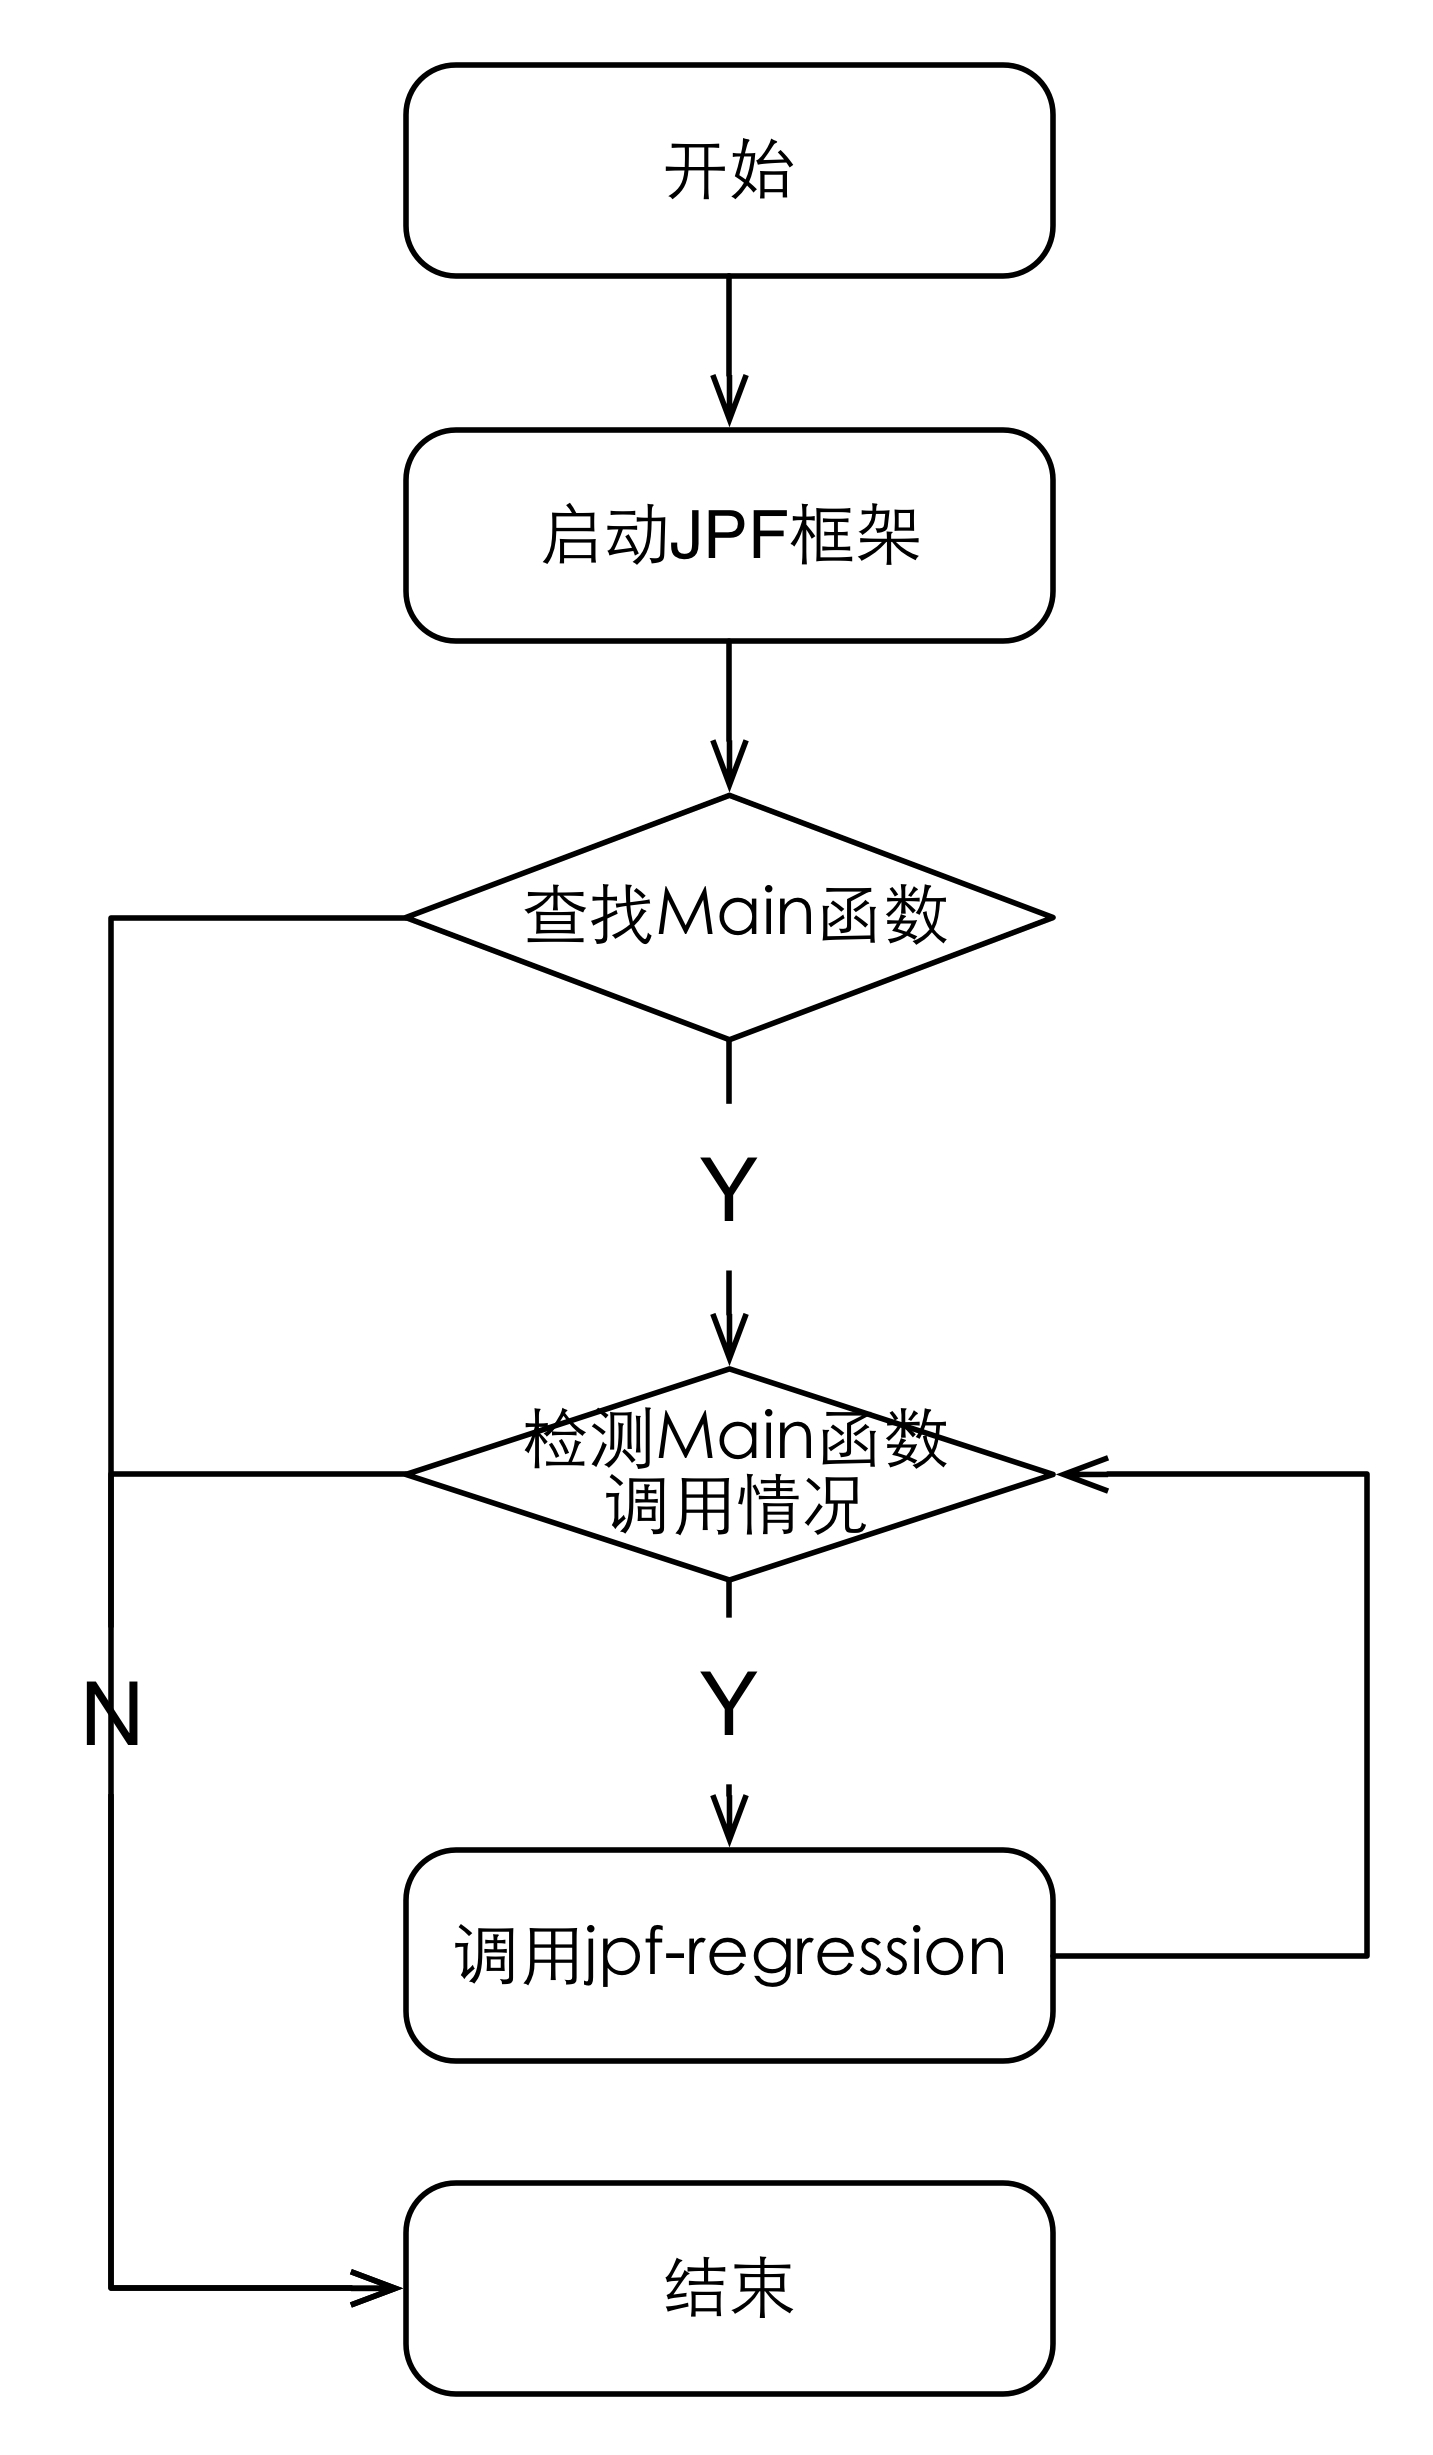
\includegraphics{chap04_jpf_launch}
	\caption {jpf框架启动流程}
	\label {impact_process}	
\end{figure}


\begin{figure}[H]
	\centering
	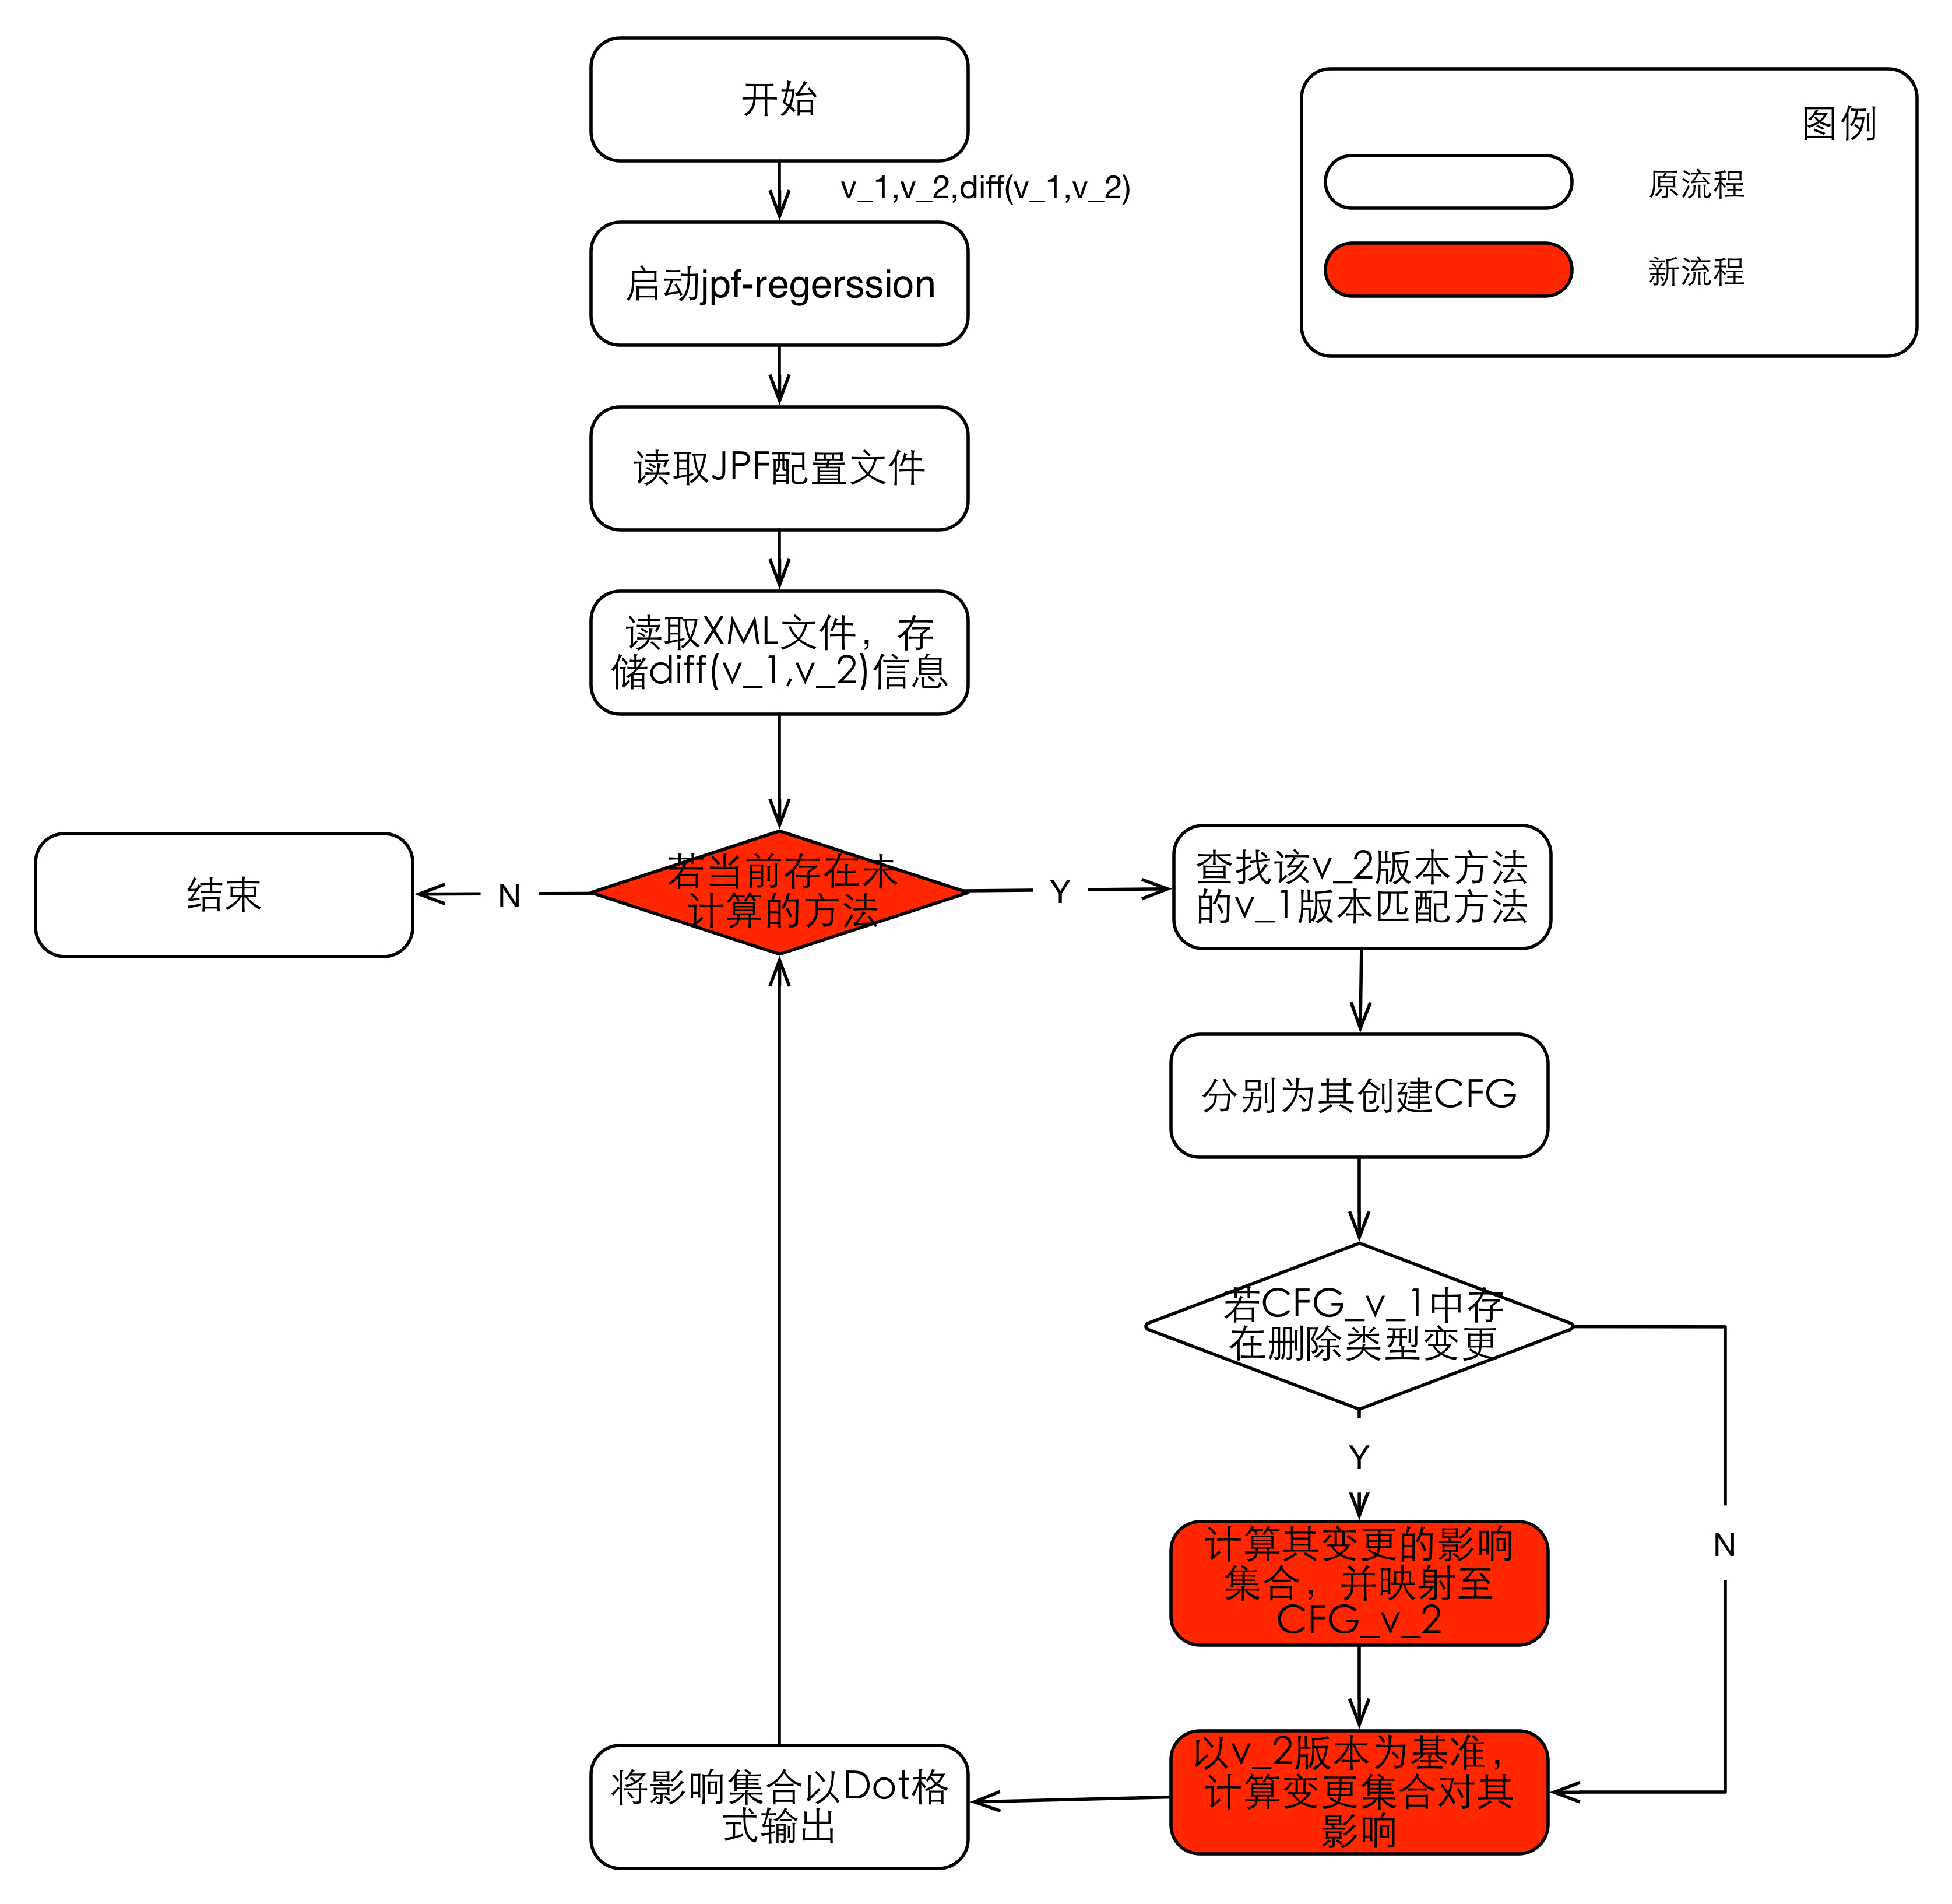
\includegraphics[width=.8\columnwidth]{chap04_jpf_old}
	\caption {jpf-regression原流程及变化}
	\label {impact_process_old}	
\end{figure}

\subsubsection{影响追踪}

在后续的兼容性分析过程中,对于得到的冲突结果,我们需要对其追根溯源,挖掘其起始的影响来源,找到对应的影响来源变更集合,以进行人工分析对比,判定该情况是否确实冲突。

因此,我们需要在变更影响分析的阶段也加入影响追踪系统的记录模块,以便记录下变更影响的轨迹,根据这些信息为后续的分析过程提供便利。

为了实现影响追踪系统,我们需要存储程序结构间的影响关系。如前所述,影响的来源主要有两类,即:
\begin{itemize}
	\item 控制依赖
	\item 数据依赖
\end{itemize}

因而,为了描述该影响关系,本文设计了Dependency类族,参见图\ref {class_depend}。该类中使用了一个二元组的数据结构depend来存储影响来源和受影响对象,并使用了多态机制来区分影响关系的类型,即是控制依赖还是数据依赖。Dependency类族中重写了hashCode()方法和equals()方法,以便能够放入集合中进行存储。

影响追踪系统中具体使用到的数据结构可以参考表\ref {track_data}。

\begin{figure}[H]
	\centering
	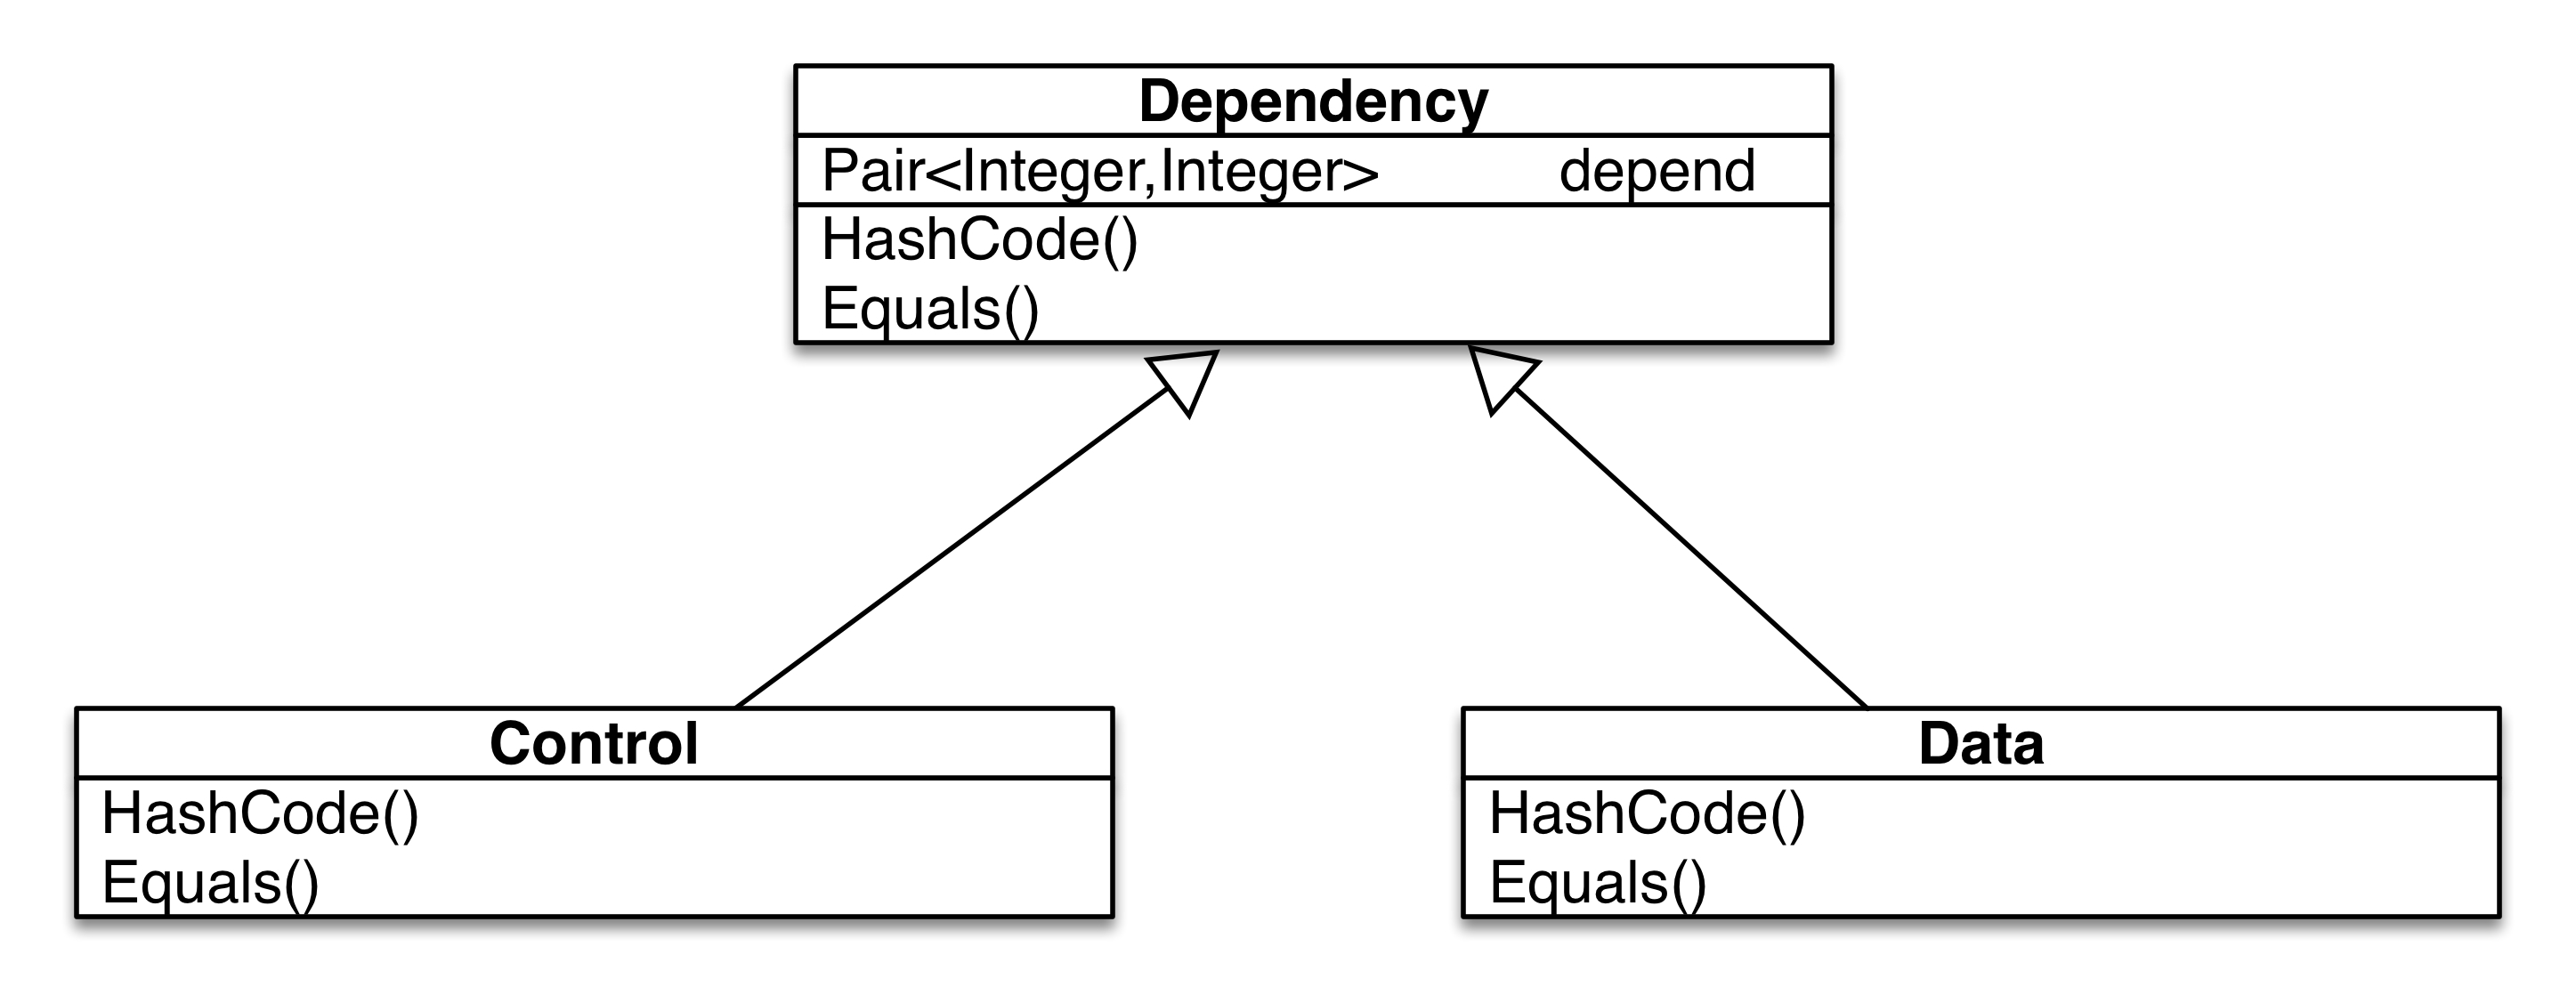
\includegraphics[width=.8\columnwidth]{chap04_depend}
	\caption {Dependency类族}
	\label {class_depend}	
\end{figure}

\begin{table}
	\caption{影响关系数据结构}
	\label{track_data}
	\centering
	\begin{tabular}{lllc}
		\toprule[1.5pt]
		{\heiti 数据类型} &{\heiti 数据结构} & {\heiti 用途} \\\midrule[1pt]
		Dependency & dependency & 单个影响关系 \\
		Control & dependency & 单个控制依赖影响关系 \\
		Data & dependency & 单个数据依赖影响关系 \\
		Map<Integer, Set<Dependency> > & depend & 存储计算过程中的全部影响关系\\
		\bottomrule[1.5pt]
	\end{tabular}
\end{table}

影响关系的创建需要在进行变更影响分析过程的同时进行,以便记录下整个影响关系链。最后将整个影响关系输出到Dot文件去即可。


\subsubsection{错误记录}

原有的jpf-regression工具由于是单次分析过程,因而一旦在运行过程中遇到问题,就会采用抛出异常终止运行的方式结束分析。然而我们在实际情况中需要进行大规模的分析作业,如果仅仅在其中单个文件的分析过程中出错就终止整个分析作业,会造成极大的时间和计算资源的浪费。

因而我们对该工具的异常处理方式进行了修改,使其在单次分析过程中如果遇到问题,则会及时抛出异常,但并不终止整个程序的运行,而采取了继续往下执行并分析其他文件的策略。然而分析错误是确实存在的,为了不丢失这类错误信息,我们为工具添加了错误记录系统,不断记录单次分析过程中遇到的问题。

我们对程序运行过程中可能出现的报错情况进行了分类,并设计了专门的错误统计类以专门别类的对错误情况进行记录和统计。该类的设计可以参考图\ref {class_error}。其中使用到的数据结构可以参考表\ref {error_data}的说明。

\begin{figure}[H]
	\centering
	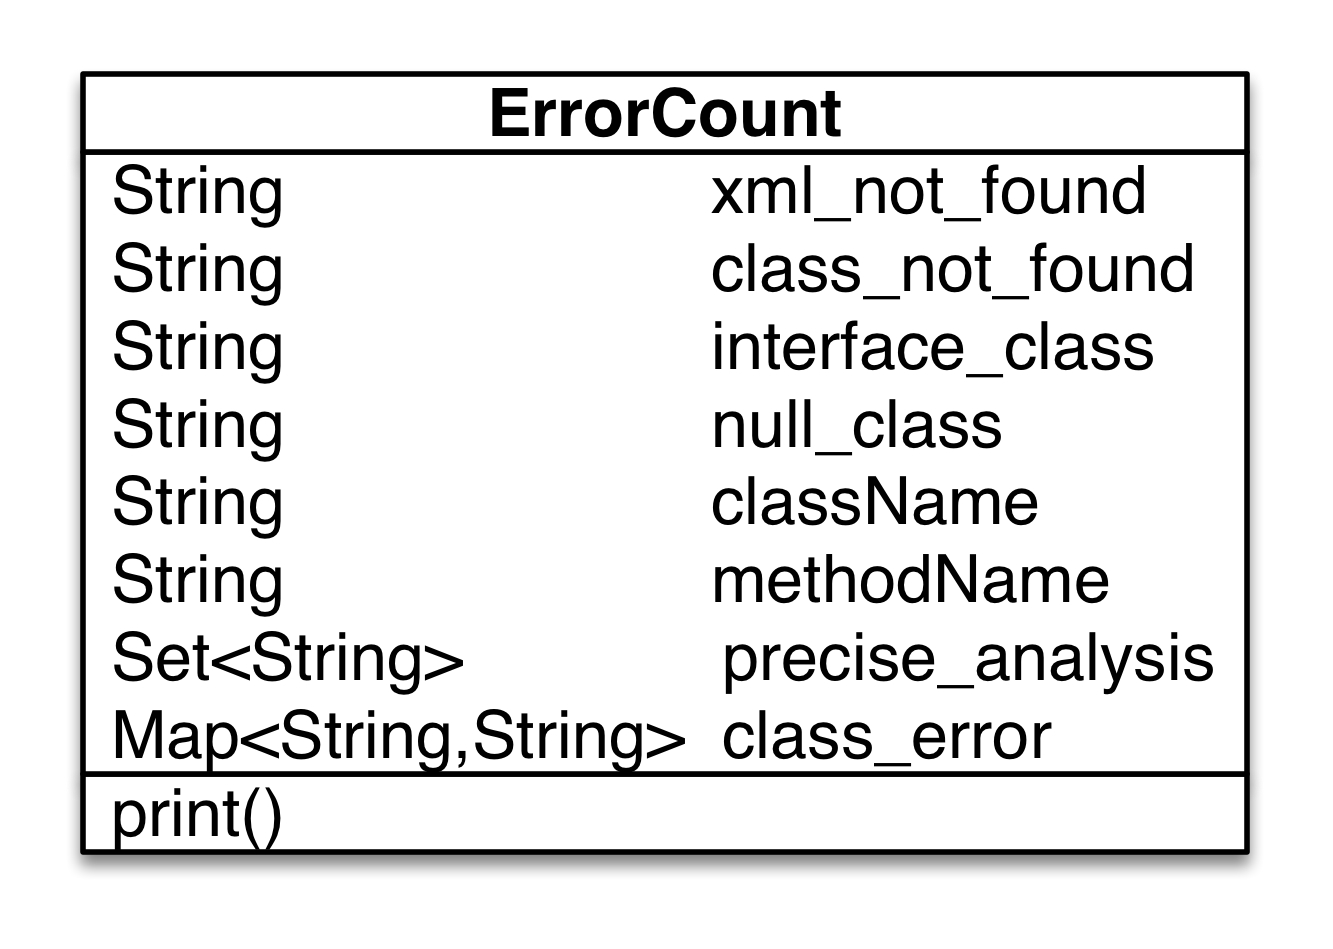
\includegraphics[width=.8\columnwidth]{chap04_error}
	\caption {ErrorCount类}
	\label {class_error}	
\end{figure}

\begin{table}
	\caption{错误记录数据结构}
	\label{error_data}
	\centering
	\begin{tabular}{lllc}
		\toprule[1.5pt]
		{\heiti 数据类型} &{\heiti 数据结构} & {\heiti 用途} \\\midrule[1pt]
		String & xml\_not\_found & 错误:XML文件未找到 \\
		String & class\_not\_found & 错误:Class文件未找到 \\
		String & interface\_class &  错误:接口类\\
		String & null\_class & 错误:类中无具体实现(如抽象类)\\
		Set<String> & precise\_analysis & 记录有多少方法在影响计算过程中出错\\
		Map<String, String> & class\_error & 记录有哪些类出现了哪些错误\\
		void & print() & 输出错误记录\\
		\bottomrule[1.5pt]
	\end{tabular}
\end{table}


\subsubsection{大规模分析}

原有的jpf-regression工具只能支持单次分析过程,在实际情况中我们需要工具具备大规模批量化分析的能力,以应对大规模软件系统的实际需求。为此我们可以保留原有的单次分析过程,然后在上层进行封装,循环多次调用单次分析过程,以达到批量化自动分析的效果。这个过程由于进行了封装,对于用户而言是透明的。

同时,在进行大规模分析的时候,输出文件的命名格式也需要修改。在原单次分析过程中,输出文件直接采用被分析的方法名进行命名。对于分析小型文件而言,这种设计就足够了,然而在大规模分析的时候,我们需要进行一定的优化。

由于大规模分析时,可能存在一些现象,例如:
\begin{enumerate}
	\item 函数重载
	\item 不同版本间的代码其方法可能无法一一匹配。例如有的方法仅在单个版本中出现。
\end{enumerate}

在这种情况下,我们采用的命名格式为:

$MethodName+HashCode(MethodName)+ExtensionName$

其中,$MethodName$由即为方法名,无法保证方法名的唯一性。再利用Java中的HashCode方法,对$MethodName$计算其HashCode作为其后缀,以保证方法名的唯一性。最后$ExtentionName$即为文件扩展名,在jpf-regression中$ExtentionName = “.dot”$。

同时我们也保留了原有的单次分析能力,以满足实际情况中的其他需要,例如进行小规模的案例分析。

其次,在进行大规模分析的情况下,由于实验数据量的庞大,我们无法按照单次分析过程中那样手动查看并分析实验结果。因此,为了适应这种需要,我们还增加了数据统计模块,使得程序具备一定的自动化分析实验结果的能力。

相关的类设计可以参考图\ref {class_run_all}和图\ref {class_run_jpf}。其中涉及的数据结构及其说明参考表\ref {run_all_data}和表\ref {run_jpf_data}。

\begin{figure}[H]
	\centering
	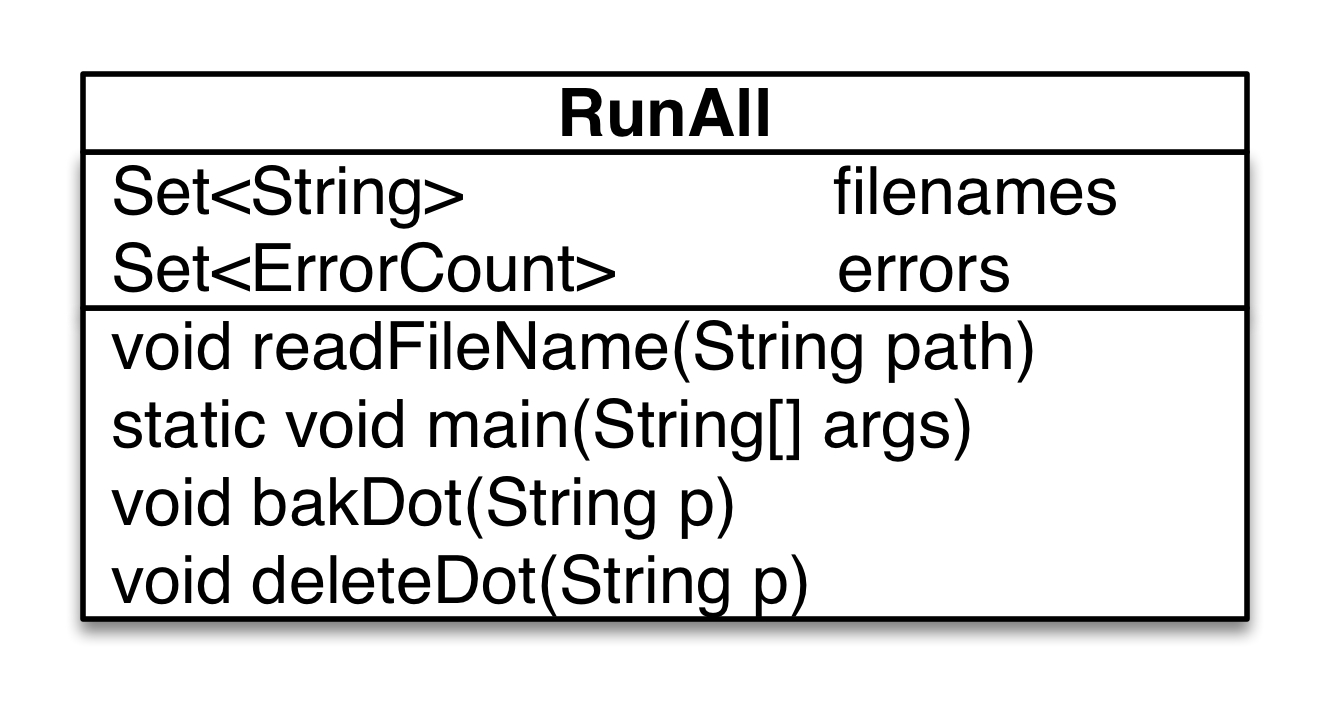
\includegraphics[width=.8\columnwidth]{chap04_run_all}
	\caption {RunAll类}
	\label {class_run_all}	
\end{figure}

\begin{figure}[H]
	\centering
	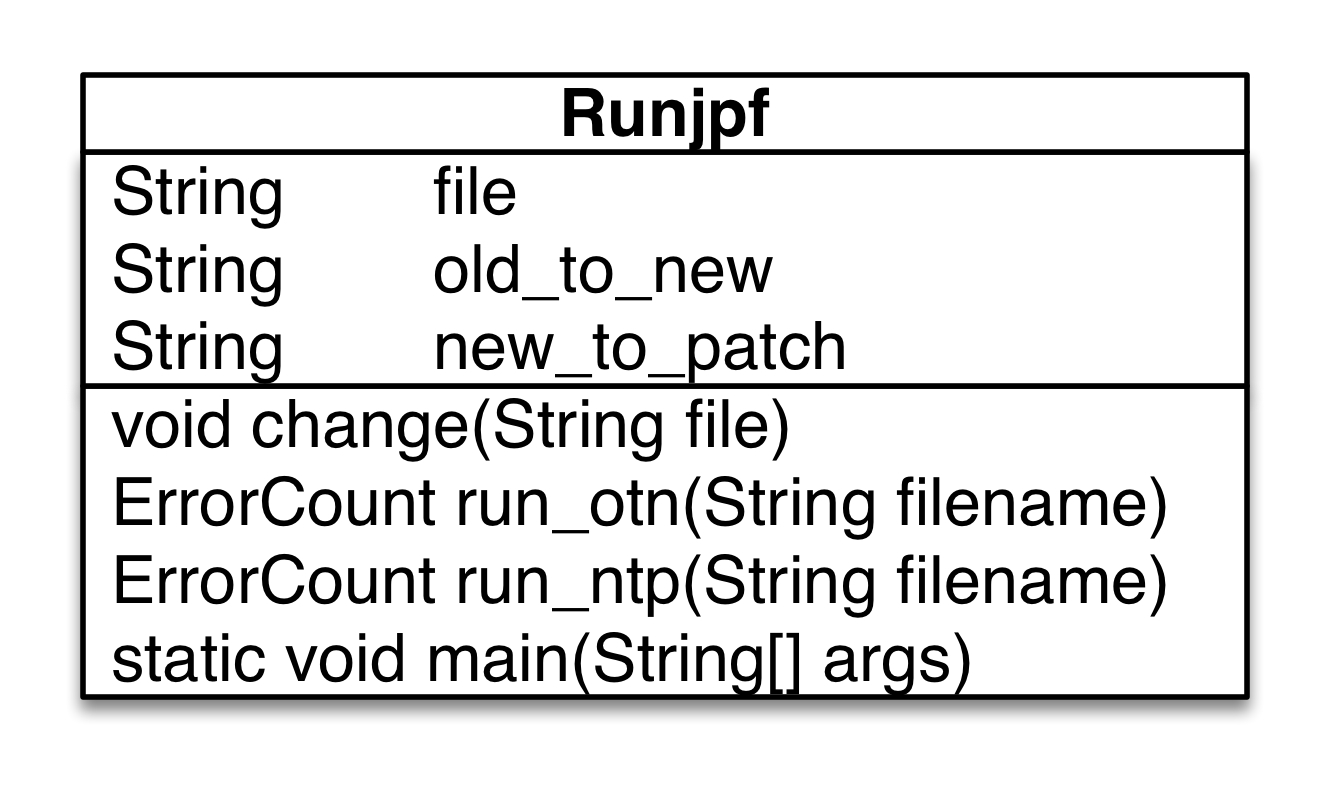
\includegraphics[width=.8\columnwidth]{chap04_run_jpf}
	\caption {Runjpf类}
	\label {class_run_jpf}	
\end{figure}

\begin{table}
	\caption{RunAll数据结构}
	\label{run_all_data}
	\centering
	\begin{tabular}{lllc}
		\toprule[1.5pt]
		{\heiti 数据类型} &{\heiti 数据结构} & {\heiti 用途} \\\midrule[1pt]
		Set<String> & filenames & 存储待分析的文件名 \\
		Set<ErrorCount> & errors & 存储每次分析中出现的错误 \\
		void & readFileName(String path) & 从文件中读取待分析的文件名\\
		static void & main(String[] args) & 实现大规模分析过程\\
		void & bakDot(String p) & 备份分析结果\\
		void & deleteDot(String p) & 删除分析结果\\
		\bottomrule[1.5pt]
	\end{tabular}
\end{table}

\begin{table}
	\caption{Runjpf数据结构}
	\label{run_jpf_data}
	\centering
	\begin{tabular}{lllc}
		\toprule[1.5pt]
		{\heiti 数据类型} &{\heiti 数据结构} & {\heiti 用途} \\\midrule[1pt]
		String & file & 待分析文件名\\
		String & old\_to\_new & $impact(diff(v_2,v_1),v_2)$过程的配置文件位置\\
		String & new\_to\_patch & $impact(diff(v_2,v_4),v_2)$过程的配置文件位置\\
		void & change(String file) & 改变当前需要读取的配置文件\\
		ErrorCount & run\_otn(String filename) & 运行$impact(diff(v_2,v_1),v_2)$过程 \\
		ErrorCount & run\_ntp(String filename) & 运行$impact(diff(v_2,v_4),v_2)$  \\
		static void & main(String[] args) & 实现单次分析过程\\
		\bottomrule[1.5pt]
	\end{tabular}
\end{table}


\subsubsection{Bug修复}

在实际使用jpf-regression进行实验的过程中,我们发现该工具存在一些Bug,这些Bug或多或少的导致了分析结果的正确性和精度降低。我们对其中力所能及的Bug进行了修复,并对这些Bug进行了总结。

目前已知的Bug及其修复情况可以参见表\ref {bug_data}。

\begin{table}
	\caption{Bug报告}
	\label{bug_data}
	\centering
	\begin{tabular}{lllc}
		\toprule[1.5pt]
		{\heiti Bug} &{\heiti 危害} & {\heiti 修复} \\\midrule[1pt]
		内部类无法进行方法匹配 & 小 & 否\\
		只有单个版本存在时无法进行方法匹配 & 小 & 是\\
		将$CFG_{v\_1}$的影响集合映射到$CFG_{v\_2}$时判断条件出错 & 大 & 是\\
		依赖JAR包jpf\_guided\_test出错 & 小 & 否\\
		依赖JAR包jpf\_symboc出错 & 小 & 否\\
		\bottomrule[1.5pt]
	\end{tabular}
\end{table}

\section{冲突分析}

如前所述,本文中给出了一个较为简单的自动化冲突分析方法,就目前而言,更精确的分析结果需要人工分析过程的辅助。

在实现冲突分析的过程中,主要涉及到的流程包括:
\begin{enumerate}
	\item 读取语义影响范围分析的结果
	\item 计算是否发生影响范围重叠
	\item 对于发生了重叠现象的影响范围,判定为冲突
	\item 回溯不兼容部分代码的影响来源并输出其影响关系链
	\item 根据得到的影响关系链,人工分析重叠部分,判定是否确实冲突
\end{enumerate}

可见,冲突分析过程中的主要工作包括:
\begin{itemize}
	\item 计算影响范围重叠
	\item 进行影响追踪,输出影响关系链
\end{itemize}

\section{本章小结}